%============================================================
%  Capitolo 6 – Normalization Layers
%============================================================
\chapter{Normalization Layers}
\label{ch:normalization}

I \textbf{layer di normalizzazione} sono componenti ormai indispensabili nelle
reti neurali profonde. Senza di essi, addestrare reti molto profonde è
difficoltoso: i gradienti esplodono o svaniscono, i tempi di convergenza si
allungano e la scelta del learning rate diventa critica. Questo capitolo
introduce il problema del \emph{covariate shift}, la soluzione più nota
(Batch Normalization), le varianti sviluppate per contesti diversi e una
discussione critica su \emph{perché} la normalizzazione funziona davvero
\citep{bishop2024}.

%------------------------------------------------------------
\section{Covariate Shift e Internal Covariate Shift}
\label{sec:covariate-shift}

Il \textbf{covariate shift} è un cambiamento nella distribuzione degli input
di un sistema di apprendimento: tipicamente la distribuzione durante il test
differisce da quella durante il training. Questo fenomeno danneggia le
prestazioni e viene normalmente affrontato con tecniche di \emph{domain
adaptation}.

Nelle reti neurali profonde esiste un fenomeno analogo ma interno:
l'\textbf{internal covariate shift}. Durante il training, gli aggiornamenti
dei pesi nei layer inferiori modificano continuamente la distribuzione degli
input per i layer superiori. I layer successivi devono quindi adattarsi non
solo a nuovi dati, ma a distribuzioni che cambiano ad ogni step di
ottimizzazione, rallentando significativamente il training.

%------------------------------------------------------------
\section{Batch Normalization}
\label{sec:batch-norm}

\subsection{Idea di Base}
\label{subsec:bn-idea}

La \textbf{Batch Normalization} (BN) \citep{ioffe2015batch} è un metodo di
normalizzazione applicato ai layer interni della rete. Normalmente gli input
alla rete vengono normalizzati nell'intervallo $[0,1]$ o $[-1,1]$ oppure
portati a media zero e varianza unitaria. BN estende questa pratica ai layer
intermedi, eseguendo un'\emph{operazione di whitening} sulle attivazioni
ad ogni step.

\subsection{Perché l'Approccio Naïf Non Funziona}
\label{subsec:naive-approach}

L'approccio banale sarebbe: addestrare su un batch, aggiornare i parametri,
poi normalizzare le attivazioni. Questo però \textbf{non funziona}: porta a
un'esplosione dei bias mentre i parametri di distribuzione (media e varianza)
rimangono invariati. Il motivo è che l'ottimizzazione con discesa del
gradiente non tiene conto della normalizzazione che avverrà al passo
successivo, ignorando sistematicamente il suo effetto.

\subsection{La Soluzione: un Layer di Normalizzazione Differenziabile}
\label{subsec:bn-layer}

La soluzione proposta da \citet{ioffe2015batch} è aggiungere un \textbf{layer
esplicito} che esegua la normalizzazione come parte del grafo computazionale,
in modo che il gradiente possa ``vedere'' la normalizzazione e fare
aggiustamenti se necessario.

\begin{figure}[H]
  \centering
  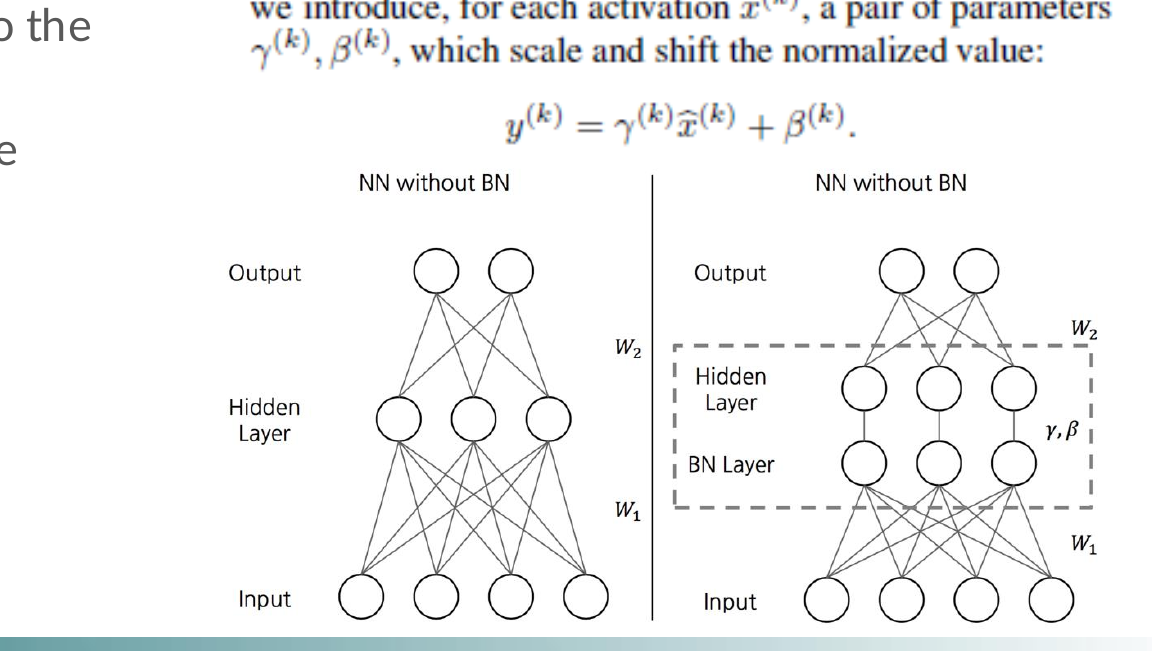
\includegraphics[width=0.72\linewidth]{figures/cf06_bn_layer_diagram.png}
  \caption{Confronto tra una rete senza BN (sinistra) e con BN (destra). Il
           BN Layer, inserito tra il layer lineare e quello successivo,
           introduce i parametri apprendibili $\gamma$ e $\beta$ che scalano
           e traslano le attivazioni normalizzate.}
  \label{fig:bn_layer_diagram}
\end{figure}

\paragraph{Algoritmo formale.}
Dato un mini-batch $\mathcal{B} = \{x_1, \ldots, x_m\}$ e i parametri
apprendibili $\gamma, \beta$, il layer BN calcola:

\begin{align}
  \mu_{\mathcal{B}}   &\leftarrow \frac{1}{m} \sum_{i=1}^{m} x_i
                       && \text{// media del mini-batch} \\[4pt]
  \sigma_{\mathcal{B}}^2 &\leftarrow \frac{1}{m} \sum_{i=1}^{m}
                           (x_i - \mu_{\mathcal{B}})^2
                       && \text{// varianza del mini-batch} \\[4pt]
  \hat{x}_i           &\leftarrow \frac{x_i - \mu_{\mathcal{B}}}
                           {\sqrt{\sigma_{\mathcal{B}}^2 + \epsilon}}
                       && \text{// normalizzazione (z-score)} \\[4pt]
  y_i                 &\leftarrow \gamma\,\hat{x}_i + \beta
                        \;\equiv\; \mathrm{BN}_{\gamma,\beta}(x_i)
                       && \text{// scala e trasla}
\end{align}

dove $\epsilon \approx 10^{-5}$ evita la divisione per zero.

\begin{figure}[H]
  \centering
  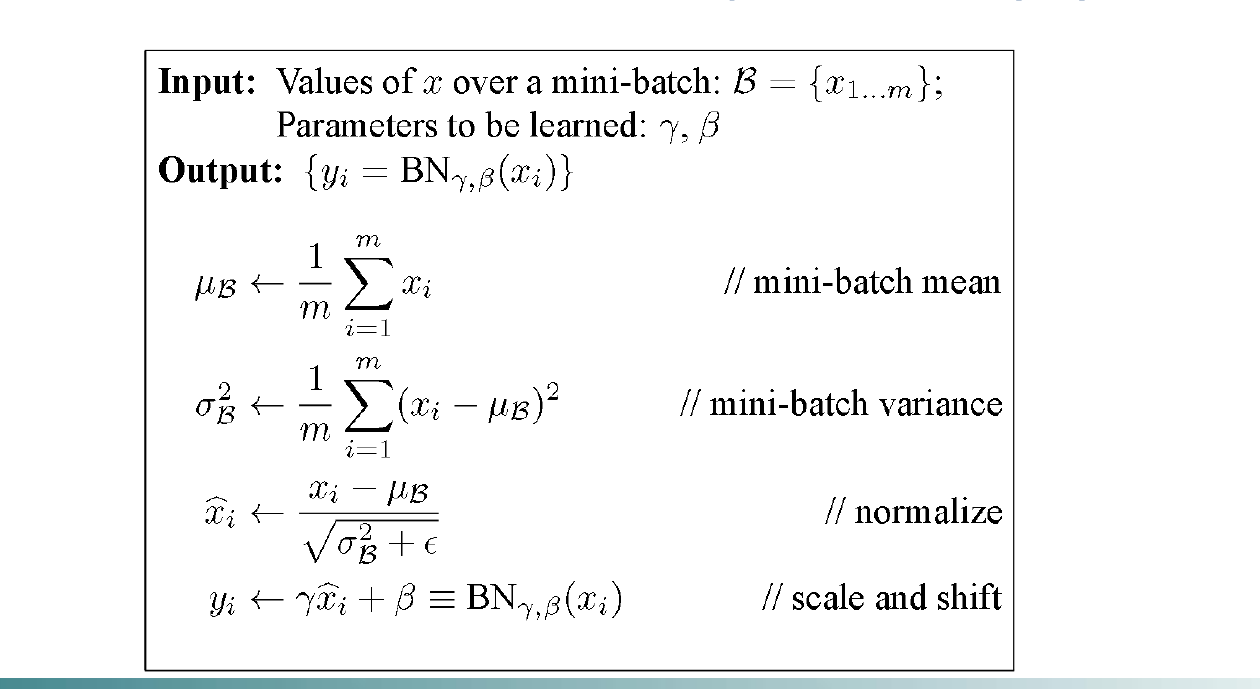
\includegraphics[width=0.62\linewidth]{figures/cf06_bn_algorithm.png}
  \caption{Pseudocodice dell'algoritmo di Batch Normalization come presentato
           nel paper originale \citep{ioffe2015batch}. Le quattro operazioni
           (media, varianza, normalizzazione, scale-and-shift) costituiscono
           il forward pass del layer BN.}
  \label{fig:bn_algorithm}
\end{figure}

\subsection{Parametri Apprendibili $\gamma$ e $\beta$}
\label{subsec:bn-gamma-beta}

Senza $\gamma$ e $\beta$, l'output del layer BN avrebbe sempre media $0$ e
deviazione standard $1$, limitando la capacità rappresentativa della rete.
I parametri $\gamma$ (fattore di scala) e $\beta$ (bias) permettono alla rete
di operare su qualsiasi range di valori.

Un aspetto cruciale è che $\gamma$ e $\beta$ \textbf{non annullano la
normalizzazione}: sono parametri appresi per discesa del gradiente e risultano
molto più stabili di $\mu$ e $\sigma$ (che cambiano ad ogni mini-batch). Il
layer ha persino la capacità di imparare la funzione identità (per
``de-normalizzare'' se necessario), ma lo fa solo se il task lo richiede.

%------------------------------------------------------------
\section{Vantaggi della Batch Normalization}
\label{sec:bn-benefits}

\subsection{Benefici Teorici (Motivazione Originale)}
\label{subsec:bn-theory}

\begin{description}
  \item[Riduzione dell'Internal Covariate Shift] La motivazione originale
        del paper. Con BN, ogni neurone tende ad avere un'attivazione
        approssimativamente gaussiana (solitamente non attivo, a volte
        parzialmente attivo, raramente molto attivo). Il covariate shift è
        indesiderabile perché i layer successivi devono continuamente
        adattarsi a cambiamenti nel \emph{tipo} di distribuzione, non solo
        nei parametri.

        \begin{tcolorbox}[colback=orange!5!white, colframe=orange!60!black,
                          title={Nota critica}]
          \textbf{Questa motivazione è stata confutata sperimentalmente.}
          Ricerche successive hanno dimostrato che BN non riduce
          significativamente l'internal covariate shift. I veri benefici
          hanno spiegazioni diverse (cfr.\ Sezione~\ref{sec:why-works}).
        \end{tcolorbox}

  \item[Riduzione di vanishing/exploding gradients] Con attivazioni
        distribuite normalmente, il segnale del gradiente si propaga in modo
        più stabile tra i layer. Senza BN, attivazioni basse in un layer
        possono propagarsi a cascata producendo attivazioni sempre più piccole
        nei layer successivi.
\end{description}

\subsection{Benefici Pratici}
\label{subsec:bn-practical}

\begin{itemize}
  \item \textbf{Riduce i tempi di training}: meno problemi di gradienti
        anomali $\Rightarrow$ convergenza più rapida.
  \item \textbf{Riduce il bisogno di regolarizzazione} (dropout, L2): le
        medie e varianze calcolate sul batch introducono rumore stocastico
        che impedisce alla rete di memorizzare le risposte corrette per ogni
        esempio (effetto implicito di regolarizzazione).
  \item \textbf{Permette learning rate più alti}: minor pericolo di
        esplosione del gradiente consente di usare $\eta$ più grandi senza
        instabilità.
  \item \textbf{Abilita funzioni di attivazione saturanti in reti profonde}:
        la normalizzazione impedisce alle attivazioni di finire nelle zone di
        saturazione della sigmoide (valori molto alti o molto bassi), dove
        il gradiente è quasi nullo.
\end{itemize}

\begin{figure}[H]
  \centering
  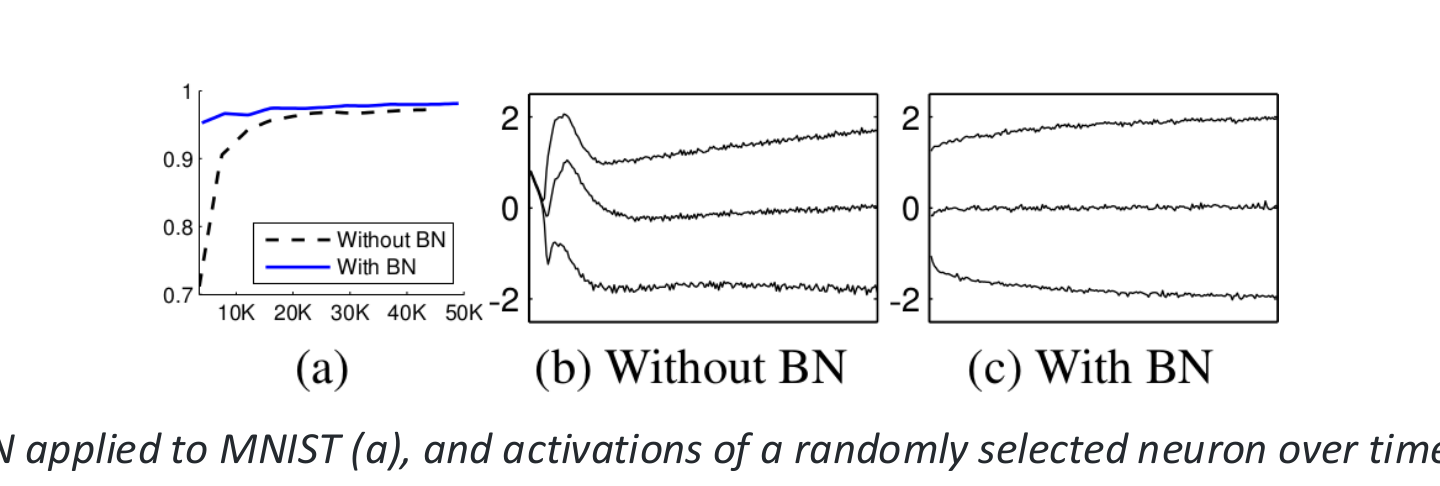
\includegraphics[width=0.82\linewidth]{figures/cf06_bn_mnist_activations.png}
  \caption{Risultati sperimentali su MNIST \citep{ioffe2015batch}.
           (a) Accuratezza durante il training: con BN si raggiunge
           convergenza più rapida e accuratezza finale più alta.
           (b) Senza BN: l'attivazione di un neurone casuale oscilla
           ampiamente nel tempo. (c) Con BN: le attivazioni si stabilizzano
           presto e rimangono nella stessa distribuzione per tutto il
           training.}
  \label{fig:bn_mnist}
\end{figure}

%------------------------------------------------------------
\section{Posizionamento del Layer BN}
\label{sec:bn-position}

Il BN layer viene tipicamente inserito \textbf{tra il layer lineare (o
convolutivo) e la funzione di attivazione}. Questa posizione permette di
normalizzare le attivazioni prima che vengano passate alla non-linearità,
evitando la saturazione.

\begin{figure}[H]
  \centering
  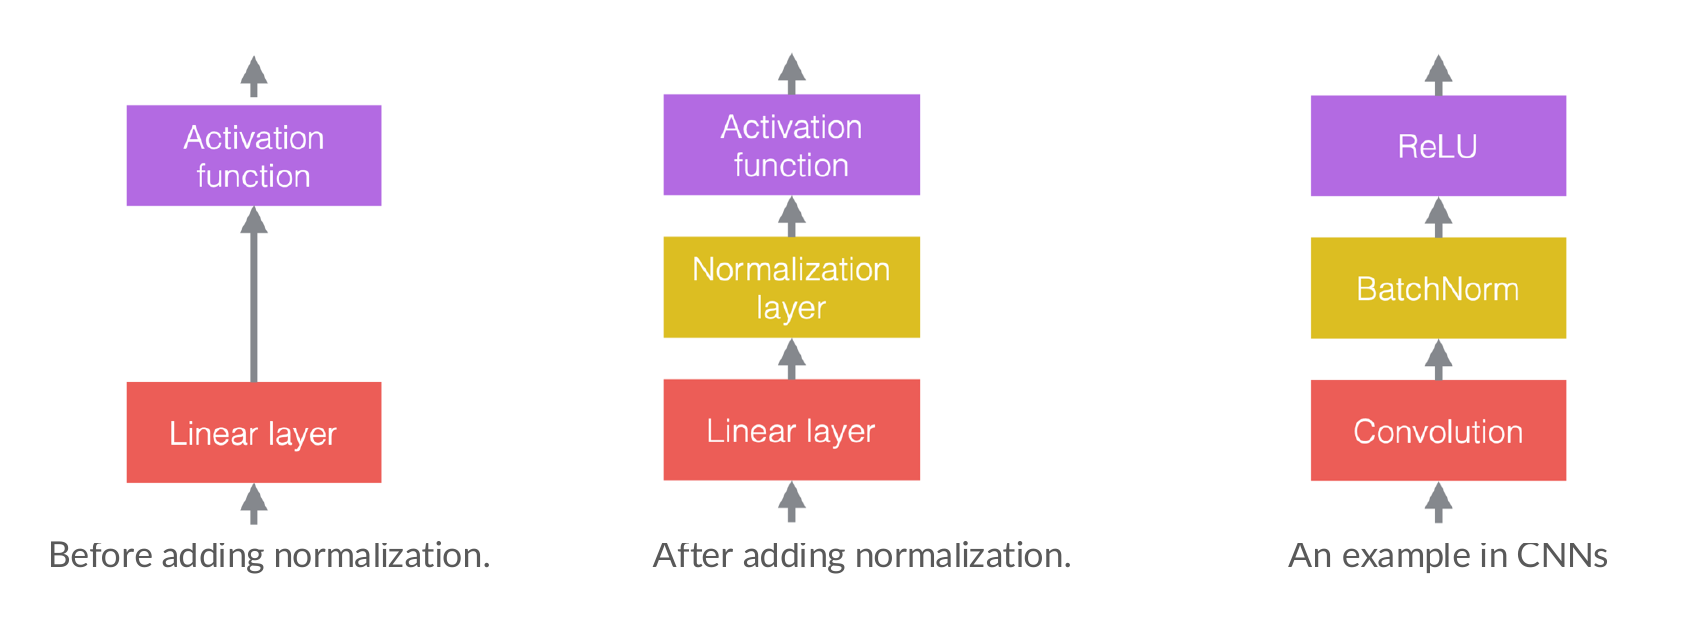
\includegraphics[width=0.82\linewidth]{figures/cf06_bn_positions.png}
  \caption{Posizionamento del layer di normalizzazione nell'architettura.
           Sinistra: rete senza normalizzazione (Linear $\to$ Activation).
           Centro: rete con normalizzazione (Linear $\to$ Norm $\to$
           Activation). Destra: esempio tipico in una CNN (Convolution $\to$
           BatchNorm $\to$ ReLU).}
  \label{fig:bn_positions}
\end{figure}

\paragraph{Fase di inferenza.}
Durante il training, $\mu$ e $\sigma^2$ vengono calcolati sul mini-batch
corrente. Durante l'inferenza, non si può usare lo stesso approccio
(il batch potrebbe contenere un solo esempio). Si usano invece le
\textbf{statistiche mobili} (running mean e running variance) accumulate
durante il training:

\begin{equation}
  \hat{\mu} \leftarrow (1 - \alpha)\,\hat{\mu} + \alpha\,\mu_{\mathcal{B}},
  \qquad
  \hat{\sigma}^2 \leftarrow (1 - \alpha)\,\hat{\sigma}^2
                             + \alpha\,\sigma_{\mathcal{B}}^2.
\end{equation}

In PyTorch questo comportamento è gestito automaticamente con
\texttt{model.train()} e \texttt{model.eval()}.

%------------------------------------------------------------
\section{Varianti di Normalizzazione}
\label{sec:norm-variants}

La scelta di \emph{quali} elementi del tensore usare per calcolare media e
varianza dà origine a diverse varianti. Per un mini-batch di $N$ immagini di
altezza $H$, larghezza $W$ e $C$ canali:

\begin{figure}[H]
  \centering
  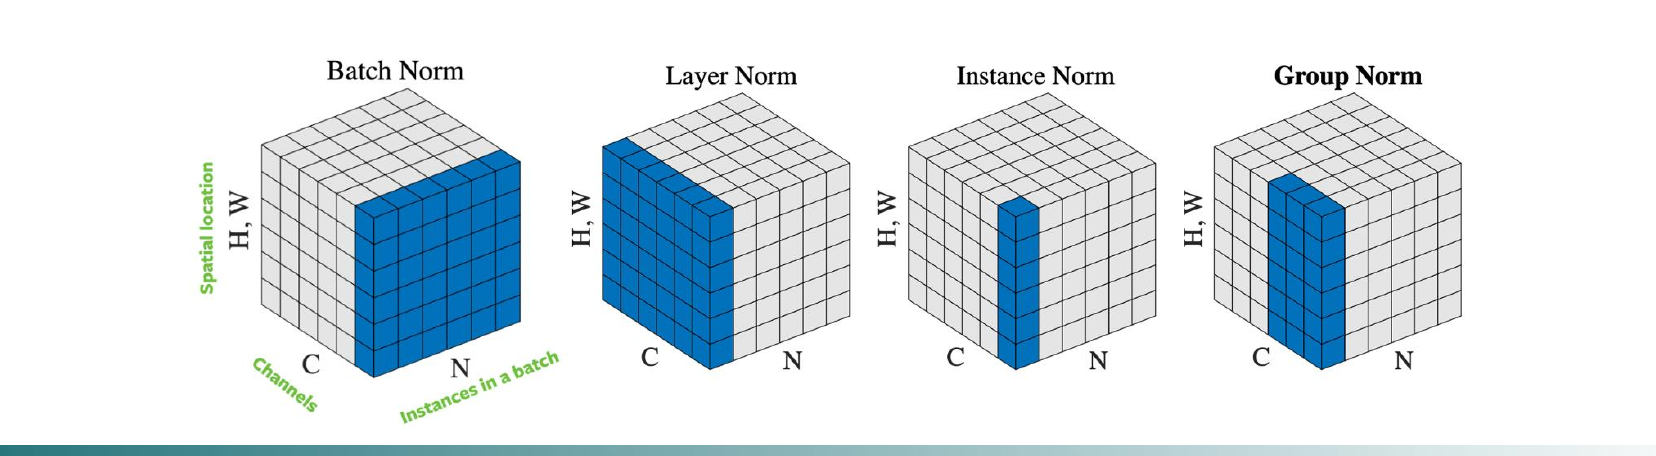
\includegraphics[width=0.90\linewidth]{figures/cf06_norm_types.png}
  \caption{Le quattro principali operazioni di normalizzazione. In blu sono
           evidenziati gli elementi usati per calcolare media e varianza per
           ogni singola statistica. Assi: $N$ (istanze nel batch), $C$
           (canali), $H \times W$ (posizioni spaziali).}
  \label{fig:norm_types}
\end{figure}

\subsection{Batch Normalization (BN)}
\label{subsec:bn-variant}

Normalizza \textbf{lungo la dimensione del batch} $N$: per ogni canale $c$,
calcola media e varianza su tutti gli elementi $(n, c, h, w)$ al variare di
$n$, $h$, $w$. Produce statistiche stabili per batch grandi ma è inadatta a
batch piccoli (le stime di $\mu$ e $\sigma$ diventano rumorose) o a sequenze
di lunghezza variabile.

\begin{equation}
  \mu_c = \frac{1}{N \cdot H \cdot W} \sum_{n,h,w} x_{n,c,h,w}, \qquad
  \sigma_c^2 = \frac{1}{N \cdot H \cdot W}
               \sum_{n,h,w} (x_{n,c,h,w} - \mu_c)^2.
\end{equation}

\subsection{Layer Normalization (LN)}
\label{subsec:layer-norm}

Normalizza \textbf{lungo i canali} per ogni singola istanza: per ogni
campione $n$, calcola media e varianza su tutti i canali e le posizioni
spaziali. Non dipende dal batch, quindi funziona perfettamente con batch di
dimensione $1$ ed è la scelta standard nei \textbf{Transformer} (dove le
sequenze hanno lunghezza variabile).

\begin{equation}
  \mu_n = \frac{1}{C \cdot H \cdot W} \sum_{c,h,w} x_{n,c,h,w}.
\end{equation}

In PyTorch: \texttt{nn.LayerNorm}.

\subsection{Instance Normalization (IN)}
\label{subsec:instance-norm}

Normalizza \textbf{per canale per istanza}: media e varianza sono calcolate
su $H \times W$ per ogni coppia $(n, c)$ indipendentemente. Utile in
\textbf{style transfer} e generazione di immagini, dove la normalizzazione
deve essere specifica per ogni immagine e ogni feature map.

\begin{equation}
  \mu_{n,c} = \frac{1}{H \cdot W} \sum_{h,w} x_{n,c,h,w}.
\end{equation}

In PyTorch: \texttt{nn.InstanceNorm2d}.

\subsection{Group Normalization (GN)}
\label{subsec:group-norm}

Compromesso tra LN e IN: divide i $C$ canali in $G$ gruppi e normalizza
ogni gruppo separatamente per ogni istanza. Non dipende da $N$ e mantiene
buone prestazioni anche con batch piccoli (es.\ $N=1$ o $N=2$ tipici in
object detection con immagini ad alta risoluzione).

\begin{equation}
  \mu_{n,g} = \frac{1}{(C/G) \cdot H \cdot W}
               \sum_{c \in \text{gruppo } g, h, w} x_{n,c,h,w}.
\end{equation}

In PyTorch: \texttt{nn.GroupNorm}. Con $G = C$ si ottiene Instance Norm;
con $G = 1$ si ottiene Layer Norm.

\begin{table}[H]
  \centering
  \caption{Confronto delle varianti di normalizzazione.}
  \label{tab:norm_comparison}
  \small
  \begin{tabular}{lllll}
    \toprule
    \textbf{Metodo} & \textbf{Calcola su} & \textbf{Dipende da $N$?}
      & \textbf{Uso tipico} & \textbf{PyTorch} \\
    \midrule
    Batch Norm   & $N, H, W$ per canale  & Sì  & CNN classifica  & \texttt{BatchNorm2d} \\
    Layer Norm   & $C, H, W$ per istanza & No  & Transformer, RNN & \texttt{LayerNorm} \\
    Instance Norm & $H, W$ per (n,c)     & No  & Style transfer  & \texttt{InstanceNorm2d} \\
    Group Norm   & gruppo di canali per istanza & No & Detection, segm. & \texttt{GroupNorm} \\
    \bottomrule
  \end{tabular}
\end{table}

%------------------------------------------------------------
\section{Perché la Normalizzazione Funziona Davvero?}
\label{sec:why-works}

Nonostante la normalizzazione funzioni bene in pratica, le ragioni della sua
efficacia sono ancora oggetto di dibattito. La motivazione originale
(riduzione dell'internal covariate shift) è stata confutata sperimentalmente.
I meccanismi attualmente più accreditati sono tre:

\begin{description}
  \item[Effetto di ottimizzazione] Le reti con layer di normalizzazione sono
        più facili da ottimizzare e permettono l'uso di learning rate più
        alti. La normalizzazione \emph{liscia} la superficie di perdita,
        rendendola più uniforme e riducendo la necessità di seguire
        direzioni di gradiente complesse.

  \item[Effetto di regolarizzazione] Le stime di media e varianza calcolate
        su un mini-batch sono \textbf{rumorose} (cambiano da batch a batch).
        Questo rumore aggiuntivo agisce come un regolarizzatore implicito,
        migliorando la generalizzazione in modo simile al dropout. La rete
        non può memorizzare valori fissi perché la normalizzazione li cambia
        ad ogni step.

  \item[Riduzione della sensibilità all'inizializzazione dei pesi] Grazie
        alla normalizzazione, l'inizializzazione dei pesi diventa meno
        critica: la distribuzione delle attivazioni viene corretta
        automaticamente al primo forward pass.
\end{description}

Come conseguenza pratica, la normalizzazione permette di essere più
``distratti'' nella progettazione: si possono combinare quasi qualsiasi
blocco architetturale e avere buone probabilità di convergenza senza dover
analizzare il condizionamento della rete.

%------------------------------------------------------------
\section{Riepilogo e Linee Guida Pratiche}
\label{sec:norm-summary}

\paragraph{Regole operative.}
\begin{enumerate}
  \item Per \textbf{CNN su immagini con batch $\geq 16$}: usare
        \texttt{nn.BatchNorm2d} dopo ogni layer conv, prima della ReLU.
        Ricordare di chiamare \texttt{model.eval()} durante l'inferenza per
        usare le running statistics.
  \item Per \textbf{Transformer e modelli sequence-to-sequence}: usare
        \texttt{nn.LayerNorm}; BN è inadatta a sequenze di lunghezza
        variabile e batch piccoli.
  \item Per \textbf{object detection / segmentazione semantica} con batch
        piccoli ($N \leq 4$): preferire \texttt{nn.GroupNorm} (tipicamente
        $G = 32$) che non degrada al calare di $N$.
  \item Per \textbf{style transfer e GAN}: \texttt{nn.InstanceNorm2d}
        normalizza per immagine, preservando le statistiche di stile
        specifiche per ciascun esempio.
  \item Non usare BN dopo layer con batch size $1$ o in presenza di
        sequenze molto corte: le stime di $\mu$ e $\sigma$ saranno
        inaffidabili.
  \item Ricordarsi che BN introduce un bias implicito per ciascun canale
        tramite $\beta$: quando BN segue un layer lineare/conv con bias, il
        bias del layer precedente è ridondante e può essere disabilitato
        (\texttt{bias=False}).
\end{enumerate}

Come sottolinea \citet{bishop2024}, i layer di normalizzazione sono oggi
parte integrante di quasi ogni architettura di successo. La loro semplicità
implementativa, unita all'impatto significativo su velocità di convergenza e
generalizzazione, li rende uno strumento imprescindibile nel toolkit del Deep
Learning moderno.
